\documentclass[a4paper]{IEEEtran}

\usepackage{ifplatform}
\usepackage{verbatim}
\usepackage{graphicx}
\usepackage{epstopdf}
\graphicspath{{../figures/}}
\epstopdfsetup{outdir=./converted/}
\usepackage{float}
\usepackage{amsmath}
\usepackage{amssymb}

% SVG Package Options
\usepackage{svg}
\svgpath{ {../figures/} }
\svgsetup{inkscapeformat=pdf} % pdf/eps/ps/png
\svgsetup{inkscapelatex=true} % true/false
\svgsetup{inkscapearea=drawing}	% drawing/page
\ifwindows
\setsvg{inkscapeexe={"C:/Program Files/Inkscape/inkscape.com"}}
\fi
%\svgsetup{inkscapedpi=300} % <integer>
\svgsetup{inkscapepath=./converted/}
%svgdir/svgpath
% 	The PDF/EPS/PS/PNG graphic files as well as the LATEX files generated by Inkscape
% 	will be located in the same directory as the corresponding SVG file.
%svgsubdir/svgsubpath
%	Within the folder of the encountered SVG file, all exported files will be located in a
%	subfolder named svg-inkscape/.
%basedir/basepath/jobdir/jobpath
%	All exported files will be located in the current working directory.
%basesubdir/basesubpath/jobsubdir/jobsubpath
%	A subfolder named svg-inkscape/ within the current working directory will be used
%	for files generated by Inkscape.
%/path/to/somewhere/
%	It is also possible to give a custom path, either relative to the current working directory (./relative/path/) or as an absolute path.
\ifpdftex
\pdfsuppresswarningpagegroup=1

\begin{document}

\title{Modelling and Control of WEDM Process for Cutting of Si-Ingots}
\author{Akshay Khadse \\ Roll No. 153079011 \\ Guide: Prof. S. V. Kulkarni}
\date{\today}
\maketitle
%\tableofcontents
%\listoffigures

\begin{abstract}
	Advancement in photovoltaics as an alternative energy medium is restricted due to the limitations in the manufacturing process of thin silicon wafers. Traditional abrasive methods lead to higher kerf (material) losses. Application of micro-drilling process of Wire Electro Discharge Machining (WEDM) is a viable alternative to such traditional methods. However, WEDM is not as well established for cutting of semiconductors as it is for metals due to the lack of electrical characterization of metal-dielectric-semiconductor conduction. This work is directed towards the fabrication of the indigenous power supply unit for such unconventional load investigations. The pulsed power supply for this purpose is designed in this work. The state space model of this power supply is derived and controller is designed for this unit.
\end{abstract}

\section{Introduction}
	Solar energy is a prominent source of renewable energy across the globe. India has aimed to reach for a 100 GW contribution from solar installations alone till 2022 \cite{mnreReport}. Silicon is the most preferred material for manufacturing the photovoltaic (PV) panels. This manufacturing process is energy intensive and thereby very costly. Extracting ingots from raw silicon accounts for 20\% of the total energy consumption throughout the process \cite{del09}. Hence, the initial cost of solar installation is higher. This can be reduced by finding better options for manufacturing silicon wafers.

	Traditionally, the two popular methods for cutting of silicon are i) Wire loose slurry method and ii) Diamond saw cutting method. These methods, being abrasive in nature, lead to micro-fractures and cracks as deep as 20 $\mu$m in the final product. Because of this, the wafer size gets limited to 180 $\mu$m \cite{sopori13}. Also, about 50\% of the ingot material is lost as kerf losses \cite{joshi10}. These methods have other disadvantages like contamination of the wafers due to the slurry, etc. \cite{moeller2015}.

	WEDM is a non contact micro-drilling process which can be used to cut free form contours from large solid metal workpieces. Experiments have shown that kerf width can be reduced from 250 $\mu$m in abrasive saw cutting to 50 $\mu$m in WEDM resulting in net material saving of 200 - 300\% \cite{dongre2015multi}. This method presents a promising alternative for application to silicon wafer manufacturing. Hence, the long term goal of this project is to optimise the manufacturing process of silicon wafers. Although this process has been demonstrated for cutting of semiconductors and even ceramics \cite{sanchez2001development}, it is not as well established for these non conventional materials as it is for the metals.

	One reason for this is the lack of electrical characterisation of metal-semiconductor-dielectric sparks. The experimentation done to investigate this has so far led to the conclusion that the spark gap VI characteristics of silicon are very different from that of the steel \cite{kane2017aps}. Hence, it is important to find a reliable model for spark gap in this setting. But, Levy and Maggi \cite{levy1990wed} demonstrated that the parameter settings given by the manufacturers are only applicable for the common steel grades.

	Hence, the available machines are inadequate to carry out further experimentation as they provide discretely spaced setting ranges. An indigenously designed power supply along with a test setup is therefore required to carry out load investigations and optimise the process of Si-ingot cutting for PV applications.

	This report summarizes the work done in design, modelling, and control of prototype power supply for Si-Ingot cutting by WEDM. The literature available in this regard is discussed in the first section, followed by the peak current mode control and direct duty ratio control procedures. In subsequent sections, the time averaging modelling methodology adopted for this purpose is discussed along with the practical considerations arising in such a design. The simulations carried out based on this work are found to be in agreement with the previous similar results for WEDM based cutting of steel.

\section{Literature Survey}

\subsection{WEDM Process}
	WEDM is a non-traditional material removal process in which a continuously travelling wire electrode made of thin tungsten, brass, or copper wire of diameter 0.05 to 0.3 mm is used. There is no direct contact between the work-piece and the wire. It is a through hole machining method capable to machine high strength and temperature resistance materials. Fig. \ref{fig:lit-1} depicts the apparatus used for the experimentation hinted earlier, which mimics the arrangement in the actual WEDM machine.

	\begin{figure}
		\centering
		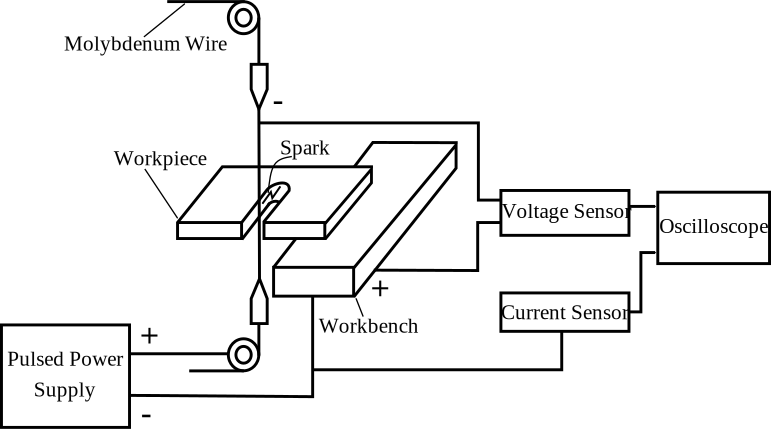
\includegraphics[width=0.45\textwidth]{wedm-diag}
		\caption{Diagrammatic representation of WEDM}
		\label{fig:lit-1}
	\end{figure}

	In WEDM, the material is eroded from the workpiece by periodic sparks occurring between the work-piece and the wire separated by the dielectric. Electrical energy from a pulsating DC power supply operating in the frequency range 20 to 30 kHz is used to generate a channel of plasma between the cathode and the anode at temperatures ranging from 8000$^\circ$ to 12000$^\circ$. Once turned off, the plasma channel breaks down, allowing the dielectric fluid to implore into the channel and flush away the molten particles and recover the dielectric strength of the gap. WEDM uses a thin wire continuously feeding through the work-piece to avoid wire breakage due to formation of localised hotspots.

	In the final product, a taper \cite{ho2004state} ranging from 15$^\circ$ for 100 mm thick to 30$^\circ$ for a 400 mm thick work-piece can be achieved. Typical Cutting Rates (CR) are 30 mm/min for 50 mm thick D2 tool steel and 750 mm/min for 150 mm thick aluminium.

\subsection{Research Areas}
	WEDM is an extensive process with a large number of parameters like pulse duration, discharge frequency, discharge current, wire feed rate, etc., which in turn affect the output product in terms of surface roughness, cutting rates and material removal rates (MRR), etc. While a lot of literature is available for steel and other metals ranging from effects of process parameters on cutting to improve the MRR, CR and surface finish, this section is concerned with presenting the relevant material available on process modelling, monitoring and control.

\subsubsection{Process Modelling}
	A theoretical model was developed by studying the influence of the work-piece material and pulse type properties of the WEDM of a work-piece with anodic property by Spur and Sch{\"o}nbeck \cite{spur1993anode} in 1993. Han et al. simulated the discharge phenomena of WEDM and developed a system which applies adaptive control to generate optimal machining condition for high precision in terms of the process parameters \cite{han2002high}.

\subsubsection{Fuzzy Control Systems}
	Fuzzy control systems have been a popular choice in this application because of independence from the requirement of comprehensive mathematical models. Kinoshita et al. investigated the effects of wire feed rate, wire winding speed, wire tension and electrical parameters on gap conditions during WEDM. Many control systems have been made based on these explicit mathematical and statistical models \cite{kinoshita1976study}. EDM pulses have been classified as open, spark, arc, off or, short on the basis of ignition delay \cite{de1982has}. Direct influence on the MRR and surface finish, electrode wear and accuracy of the final product dimensions has also been established.

\subsubsection{Wire Breakage Avoidance}
	Kinoshita et al. observed that the rapid rise in the pulse frequency of the gap voltage before the wire breakage \cite{kinoshita1982control}. They developed a monitoring system that switches off the pulse generator and servo when such pulses arise thus preventing the wire from breaking. The increase in localised temperature due to a concentration of electrical discharges at certain points of wire leads to its breakage over time. An adaptive control system for detection of the spark location and reduction of discharge energy was developed \cite{kunieda1990line}.

\subsubsection{Wire lag and wire vibration}
	Duaw and Beltrami \cite{dauw1994high} used an optical sensor for on-line monitoring the wire position and a controller for high speed. It has also been proposed to increase the gap distance to prevent wire gauging and breakage on high curvature areas of the work-piece \cite{wang2003computer} and many contour planning systems for WEDM apply this today. Several mathematical models have been derived from analysing the transient response of wire vibration based on the force acting on the tool \cite{mohri1998system}.

\subsubsection{Adaptive control systems}
	Much of the work uses adaptive control systems in this field for maintenance scheduling, machining variable height workpieces and predicting the thermal overload. Change in the work-piece thickness during machining leads to an increase in wire thermal density and breakage \cite{kinoshita1982control}. An adaptive control system was proposed with a multiple input model that monitors and controls sparking frequency according to on-line identified work-piece height by Rajurkar et al. \cite{rajurkar1997wedm}

\section{Power Supply Design}
	Power supply for the WEDM process delivers intermittent current and voltages across the electrode-dielectric-silicon ingot assembly. The pulsed nature of this power supply makes the design for such circuit difficult. This section describes the working of an ideal power source for the WEDM process of which the practical implementation is discussed in the subsequent sections.

\subsection{Working Principle}
	Fig. \ref{fig:working-1} represents the functional configuration of a pulsed power supply in which an ideal current source $I_o$ and ideal voltage source $V_o$ are connected in parallel across the spark gap load $E$. The current and voltage waveforms across the load are shown in Fig. \ref{fig:working-2}

	\begin{figure}
		\centering
		\includesvg[width=0.45\textwidth]{rep-diag-master}
		\caption{Representative diagram of ideal WEDM power supply}
		\label{fig:working-1}
	\end{figure}

\subsubsection{\textbf{t$_0$ to t$_1$}}
	During times $t=t_0$ and $t=t_1$, the current source causes the diode $D$ to turn on and $I_o$ flows through $D$ to the ideal voltage source $V_o$. The voltage across the load terminals is $V_o$ because $D$ remains in a conduction state from $t_0$ to $t_1$. This application of voltage across the spark gap terminals causes the gap to break down at $t=t_1$. This breakdown delay time depends on the dielectric strength and the magnitude of the applied voltage.

\subsubsection{\textbf{t$_1$ to t$_2$}}
	Due to breakdown of dielectric, current $I_o$ starts flowing through the spark gap $E$ and the diode $D$ turns off. If the spark gap is modelled as resistive, the voltage across terminals is $V_{dis}$ and is equal to $I_or_{gap}$. The silicon ingot now erodes along the length of moving wire electrode.
\subsubsection{\textbf{t$_2$ to t$_3$}}
	To increase the material removal rate, the spark is not allowed to become a sustained arc. This is achieved closing the switch $S$ at time $t=t_2$. When $S$ is closed, the current $I_o$ flows through current source and switch and dielectric strength of the medium is recovered by flushing fresh dielectric over the gap.

	When the gap is fully recovered, a new machining cycle is started at time $t=t_3$ by opening the switch $S$. The erosion takes place for about 10\% of the entire machining period. Thus, the power is supplied to load only for this fraction of the machining period.

	\begin{figure}
		\centering
		\includesvg[width=0.45\textwidth]{working-wf-master}
		\caption{Load voltage and current of WEDM power supply operation}
		\label{fig:working-2}
	\end{figure}

\subsection{Converter Topology}

	\begin{figure}
		\centering
		\includesvg[width=0.45\textwidth]{conv-top-master}
		\caption{Converter topology for WEDM power supply}
		\label{fig:working-3}
	\end{figure}

	This section describes the practical implementation of the ideal current and voltage sources depicted in Fig. \ref{fig:working-1}. One realisation of such power supply is proposed by Tastekin et al. in \cite{tastekin2009novel} in which a single quadrant and a two quadrant DC-DC converter is connected to the same DC link. A single quadrant converter is used as current source by controlling the inductor current and removing the filter capacitance. The voltage source is realised by controlling the output voltage of the two quadrant converter. Fig. \ref{fig:working-3} depicts this configuration using high frequency MOSFETs.

	Constant voltage of $V_o$ is maintained at the load terminals of the two quadrant converter. However, when switch $S$ in Fig. \ref{fig:working-1} is opened, the current $I_o$ goes through $D$ to the capacitor of the two quadrant converter. This acts as a disturbance to the voltage source controller and must be rejected at the earliest to maintain the constant voltage across the load terminals.

	This implementation does not use transistors and resistors, hence the only losses incurred are the switching and conduction losses of the MOSFETs, and the inductor copper losses.

\section{Converter Modelling}
	The power supply depicted in Fig. \ref{fig:working-3} is composed of three components viz. single quadrant converter acting as current source, two quadrant converter acting as voltage source, and the ignition switch. A controller is required for single quadrant and two quadrant converters, hence the state space model for these converters is found out. This section explains the time averaging method to arrive at the small signal models between the output voltage or current and the duty ratio of the switches for both the converters.

\subsection{Voltage Source}

	\begin{figure}
		\centering
		\includesvg[width=0.45\textwidth]{buck-2}
		\caption{Simplified circuit of two quadrant converter which is used as voltage source}
		\label{fig:working-4}
	\end{figure}

	Fig. \ref{fig:working-4} represents the simplified circuit for the two quadrant converter which is to be, hence the small signal transfer function $\dfrac{\hat{v}_o}{\hat{d}}$ is to be found out. The current through the inductor $L_2$ and the voltage across capacitor $C_2$ are considered as the state variables.

	When the switch $Q_2$ is on i.e. for time $DT_s$, current flows though $V_d$, $Q_2$, $r_{L_2}$, $L_2$, $r_{C_2}$ and $C_2$. Applying Kirchhoff's Voltage Law along this path gives

	\begin{equation}
		V_d - L_2 \dot{x}_1 - r_{L_2}x_1 - r_{C_2}x_1-x_2 = 0
		\label{eq:mod1}
	\end{equation}

	From current through the inductor and the capacitor is same, therefore

	\begin{equation}
		x_1 = C_2\dot{x_2} 
		\label{eq:mod2}
	\end{equation}

	The output voltage is

	\begin{equation}
		V_o = r_{C_2}x_1 + x_2
		\label{eq:mod3}
	\end{equation}

	Therefore,

	\begin{equation}
		\begin{split}
		\dot{x}_1 &= -\dfrac{r_{L_2}+r_{C_2}}{L_2}x_1 -\dfrac{1}{L_2}x_2+\dfrac{1}{L_2}V_d\\
		\dot{x}_2 &= \dfrac{1}{C_2}x_1\\
		V_o &= r_{C_2}x_1 + x_2
		\end{split}
		\label{eq:mod4}
	\end{equation}

	When $Q_2$ is off i.e. for time $(1-D)T_s$, current flows through  $D_3$, $r_{L_2}$, $L_2$, $r_{C_2}$ and $C_2$. Applying Kirchhoff's Voltage Law along this path gives

	\begin{equation}
		- L_2 \dot{x}_1 - r_{L_2}x_1 - r_{C_2}x_1-x_2 = 0
		\label{eq:mod5}
	\end{equation}

	Also,

	\begin{equation}
		x_1 = C_2\dot{x_2} 
		\label{eq:mod6}
	\end{equation}
	
	The output voltage is

	\begin{equation}
		V_o = r_{C_2}x_1 + x_2
		\label{eq:mod7}
	\end{equation}

	Therefore,

	\begin{equation}
		\begin{split}
			\dot{x}_1 &= -\dfrac{r_{L_2}+r_{C_2}}{L_2}x_1 -\dfrac{1}{L_2}x_2\\
			\dot{x}_2 &= \dfrac{1}{C_2}x_1\\
			V_o &= r_{C_2}x_1 + x_1
		\end{split}
		\label{eq:mod8}
	\end{equation}

	Constructing the state vector $x$ as

	\begin{equation}
		x =
		\begin{bmatrix}
			x_1\\x_2
		\end{bmatrix}
		\label{eq:mod9}
	\end{equation}

	In equation \eqref{eq:4}, let

	\begin{equation}
		A_1=
		\begin{bmatrix}
			-\dfrac{r_{L_2}+r_{C_2}}{L_2} & -\dfrac{1}{L_2}\vspace*{2mm}\\
			\dfrac{1}{C_2} & 0
		\end{bmatrix}
		\quad
		B_1=
		\begin{bmatrix}
			\dfrac{1}{L_2} \vspace*{2mm}\\ 0
		\end{bmatrix}
		\quad
		C_1 =
		\begin{bmatrix}
			r_{C_2} & 1
		\end{bmatrix}
		\label{eq:mod10}
	\end{equation}

	Therefore,
	
	\begin{equation}
		\begin{split}
			\dot{x} &= A_1 x + B_1 V_d\\
			V_o &= C_1 x
		\end{split}
		\label{eq:mod11}
	\end{equation}

	In equation \eqref{eq:5}, let

	\begin{equation}
		A_2=
		\begin{bmatrix}
			-\dfrac{r_{L_2}+r_{C_2}}{L_2} & -\dfrac{1}{L_2}\vspace*{2mm}\\
			\dfrac{1}{C_2} & 0
		\end{bmatrix}
		\quad
		B_2=
		\begin{bmatrix}
			0 \vspace*{2mm}\\ 0
		\end{bmatrix}
		\quad
		C_1 =
		\begin{bmatrix}
			r_{C_2} & 1
		\end{bmatrix}
		\label{eq:mod12}
	\end{equation}

	Therefore,

	\begin{equation}
		\begin{split}
			\dot{x} &= A_1 x + B_1 V_d\\
			V_o &= C_1 x
		\end{split}
		\label{eq:mod13}
	\end{equation}

	Equation \eqref{eq:mod11} is valid for $dT_s$ and equation \eqref{eq:mod13} is valid for $(1-d)T_s$. Time averaging equations \eqref{eq:mod11} and \eqref{eq:mod13} leads to

	\begin{equation}
		\begin{split}
			\dot{x} &= [dA_1+(1-d)A_2]x + [dB_1 + (1-d)B_2]V_d\\
			V_o &= [dC_1+(1-d)C_2]x
		\end{split}
		\label{eq:mod14}
	\end{equation}

	Small signal transfer function for this representation is derived by introducing small perturbations in $x$, $V_o$, and $d$ and eliminating the steady state quantities. Complete mathematical treatment is described in appendix \ref{app:modelling}. The small signal transfer function of the output voltage of two quadrant converter with respect to the duty ratio of the switch $Q_2$ turns out to be

	\begin{multline}
		\therefore \dfrac{\hat{v}_o(s)}{\hat{d}(s)} = C[sI-A]^{-1}[(A_1-A_2)X+(B_1-B_2)V_d]\\+(C_1-C_2)X
		\label{eq:mod27a}
	\end{multline}

	The bode plot for this transfer function when the values of inductors and capacitors are chosen as described in section \ref{sec:practical-considerations} is shown in Fig. \ref{fig:uncomp-vs}

	\begin{figure}
		\centering
		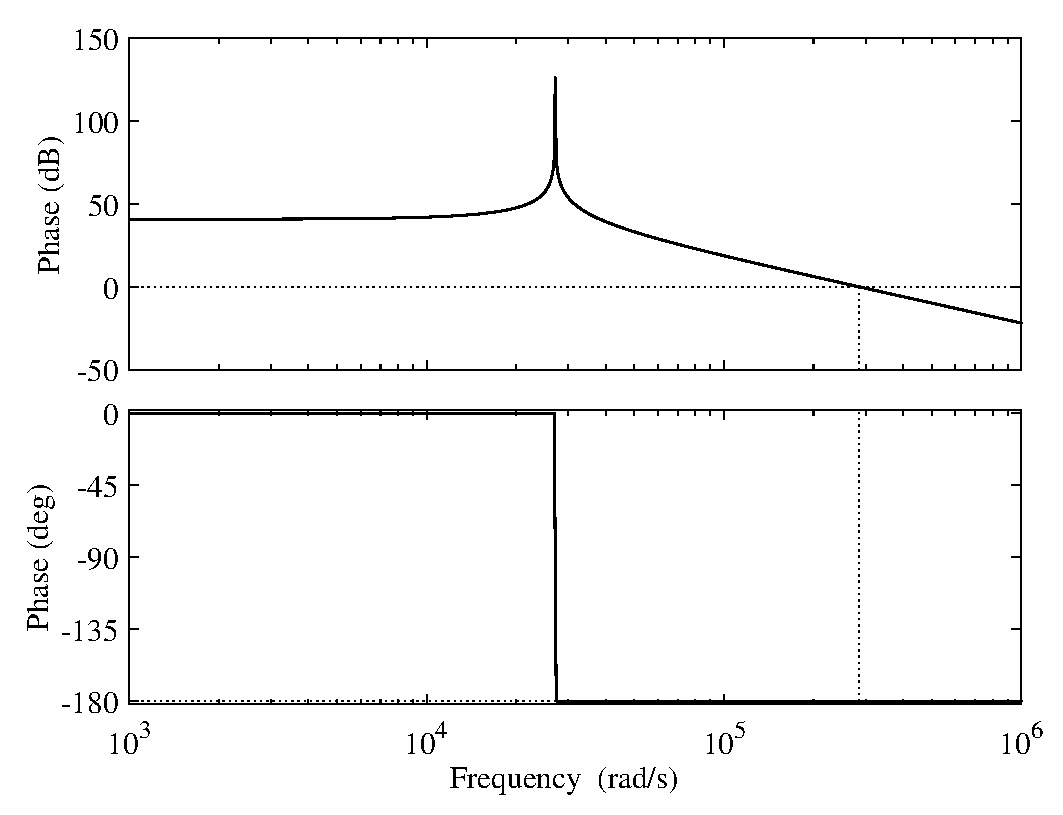
\includegraphics[width=0.45\textwidth]{uncompensated-vs}
		\caption{Bode plot of uncompensated transfer function of voltage source; Gm = $\infty$,  Pm = 0.0166$^\circ$ (at 2.85e+05 rad/s)}
		\label{fig:uncomp-vs}
	\end{figure}

\subsection{Current Source}

	\begin{figure}
		\centering
		\includesvg[width=0.45\textwidth]{buck-1-master}
		\caption{Simplified circuit of single quadrant converter which is used as current source}
		\label{fig:working-5}
	\end{figure}

	Similar approach is applied for finding out the transfer function of the output current with respect or the duty cycle of the switch $Q_1$ for the single quadrant converter. Fig. \ref{fig:working-5} shows the simplified circuit diagram for the same. The current through the inductor $L_1$ is the only state variable in this case.

	When the switch $Q_1$ is on i.e. for time $dT_s$, current flows though $V_d$, $Q_1$, $r_{L_1}$, $L_1$ and $R_L$. Applying Kirchhoff's Voltage Law along this path gives
	
	\begin{equation}
		V_d - L_1 \dot{x} - r_{L_1}x - R_Lx = 0
		\label{eq:mod28}
	\end{equation}
	
	The output current is
	
	\begin{equation}
		I_o = x
		\label{eq:mod29}
	\end{equation}

	Therefore,
	
	\begin{equation}
		\begin{split}
			\dot{x} &= -\dfrac{r_{L_1}+R_L}{L_2}x +\dfrac{1}{L_2}V_d\\
			I_o &= x	
		\end{split}
		\label{eq:mod30}
	\end{equation}

	When $Q_1$ is off i.e. for time $(1-d)T_s$, current flows through  $D_1$, $r_{L_1}$, $L_1$ and $R_L$. Applying Kirchhoff's Voltage Law along this path gives
	
	\begin{equation}
		- L_1 \dot{x} - r_{L_1}x - R_Lx = 0
		\label{eq:mod31}
	\end{equation}
	
	The output current is
	
	\begin{equation}
		I_o = x
		\label{eq:mod32}
	\end{equation}
	
	Therefore,
	
	\begin{equation}
			\begin{split}
			\dot{x} &= -\dfrac{r_{L_1}+R_L}{L_2}x\\
			I_o &= x
		\end{split}
		\label{eq:mod33}
	\end{equation}
	
	Therefore,
	
	\begin{equation}
		\begin{split}
			A_1 &= -\dfrac{r_{L_1}+R_L}{L_1} = A_2\\
			B_1 &= \dfrac{1}{L_1} \quad B_2 = 0\\
			C_1 &= 1 = C_2
		\end{split}
		\label{eq:mod34}
	\end{equation}
	
	The transfer function $\dfrac{\hat{i}_o}{\hat{d}}$ is obtained using equations \eqref{eq:mod34} in 
	
	\begin{multline}
		\dfrac{\hat{i}_o(s)}{\hat{d}(s)} = C[sI-A]^{-1}[(A_1-A_2)X+(B_1-B_2)V_d]\\+(C_1-C_2)X
		\label{eq:mod35}
	\end{multline}
	
	where
	
	\begin{align}
		A &= A_1d+A_2(1-d)\\
		\label{eq:mod36}
	\end{align}

	The bode plot for this transfer function when the values of inductors and capacitors are chosen as described in section \ref{sec:practical-considerations} is shown in Fig. \ref{fig:uncomp-cs}

	\begin{figure}
		\centering
		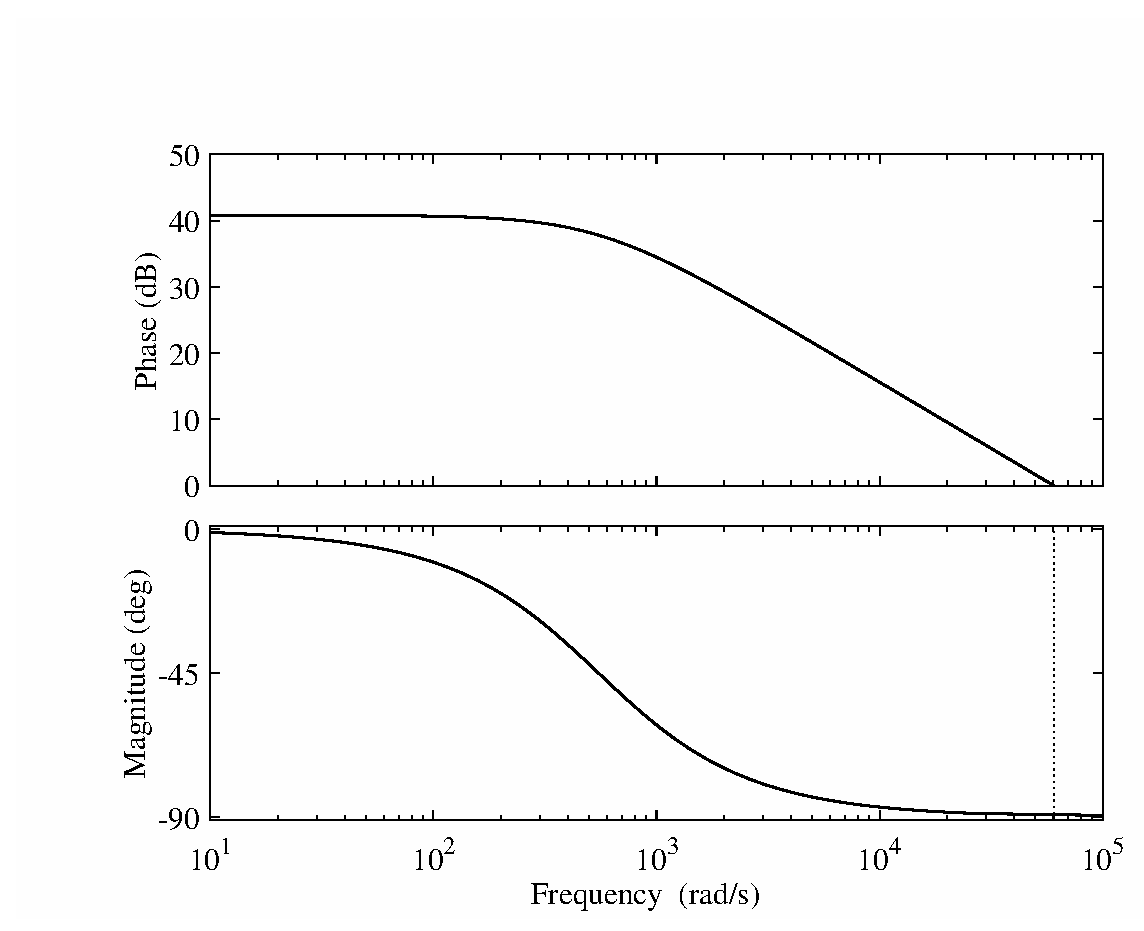
\includegraphics[width=0.45\textwidth]{uncompensated-cs}
		\caption{Bode plot of uncompensated current source transfer function; Gm = $\infty$,  Pm = 90.5$^\circ$ (at 6.05e+04 rad/s)}
		\label{fig:uncomp-cs}
	\end{figure}

\section{Controller Design}
	The dielectric strength of deionized water is around 70 MV/m. Therefore, if the gap is 1$\mu$m, minimum voltage of 70 V is required to ensure the sparking. Keeping a sufficient margin, the control objectives for the power supply are as follows
	
	\begin{enumerate}
		\item Voltage source must maintain a voltage $V_{\text{ref}}$ i.e. 80 V across its load terminals while rejecting load current disturbances up to $I_{\text{ref}}$ i.e. 10 A.
		\item Current source must provide a current of 10 A.
		\item Generating switching signal for $Q_d$ to control the erosion time during each machining cycle 
	\end{enumerate}

	The control objectives mentioned above are to be achieved by designing a scheme for switching the appropriate devices such that the aforementioned criteria is satisfactorily met. A PI controller was implemented and tuned using trial and error initially. However, this section describes a more systematic approach of compensator design based on the frequency response of the small signal transfer functions derived earlier. Automated K Factor approach \cite{muhamad2005design} used conventionally for power electronic converters was found inadequate in this case. The removal of capacitor in current source and the load from the voltage source lead to different models than those for which this approach has been tested. Hence, the compensator design criteria is discussed in this section. This section also describes a relatively advantageous technique of current mode control.

\subsection{Direct Duty Ratio Control}
	 A simple method to achieve this goal is varying the duty cycle of a pulse width modulated (PWM) signal with fixed frequency $F_s$. $F_s$ is the switching frequency of the MOSFETs used in the converters. A feedback loop is constructed by using a lead-lag compensator for this purpose as shown in Fig. \ref{fig:dirduty-1}.

	\begin{figure}
		\centering
		\includesvg[width=0.45\textwidth]{direct-duty}
		\caption{Block diagram of direct duty ratio control of single quadrant converter}
		\label{fig:dirduty-1}
	\end{figure}

	For two quadrant converter, since the control objective is tracking the reference voltage $v_{\text{ref}}$, the output voltage $v(t)$ is sensed. $v(t)$ is compared with $v_{\text{ref}}$ to obtain the error signal. This error signal is the representative of the deviation of current state of the system from the desired state. The design procedure followed is described next.

	To improve the transient response gain crossover frequency $\omega_{gc}$ should be as high as possible but approximately an order on magnitude below the switching frequency to allow the power supply to respond quickly to the transients. This was chosen as

	\begin{equation}
		\omega_{\text{cross}} = \dfrac{2 \pi F_s}{10}
		\label{eq:50}
	\end{equation}

    Also, the desirable range of phase margin is 45 to 60$^\circ$ \cite{book:768263}. Let the desired phase margin be $PM_{des}$.
    Phase that has to be added to the system is 

    \begin{equation}
    \phi_{m_1} = PM_{des} -\left(180 + \phi_{\text{OL}}\Bigr|_{\omega = \omega_{\text{cross}}}\right)
	\label{eq:50a}    
    \end{equation}

    The general form of compensator is 

    \begin{equation}
    	G_{\text{lead}} = \dfrac{1+a_1T_1s}{1+T_1s}
	    \label{eq:51}    
    \end{equation}

    where $a_1>1$

    The maximum phase lead due to this compensator is given by

    \begin{equation}
    	\phi_{m_1} = \sin^{-1}\left(\dfrac{a_1-1}{a_1+1}\right)
	    \label{eq:52}    
    \end{equation}

    This phase lag is added in between the corner frequencies $\dfrac{1}{T_1}$ and $\dfrac{1}{a_1T_1}$ and is maximum at

    \begin{equation}
    	\omega_{m_1} = \dfrac{1}{T_1\sqrt{a_1}}
	    \label{eq:53}    
    \end{equation}

    Thus, to make phase margin as desired at the gain crossover frequency as decided, $T_1$ and $a_1$ are chosen as

    \begin{equation}
		\begin{split}
			a_1 &= \dfrac{1+\sin(\phi_{m_1})}{1-\sin(\phi_{m_1})}\\
			T_1 &= \dfrac{1}{\omega_{m_1}\sqrt{a_1}}		
		\end{split}
		\label{eq:54}    
    \end{equation}

    To reduce the steady state error, a lag compensator $G_{\text{lag}}$ is required such that $\omega_{m_2} << \omega{\text{cross}}$. In the general form

    \begin{equation}
    	G_{\text{lag}} = \dfrac{1+a_2T_2s}{1+T_2s}
	    \label{eq:55}    
    \end{equation}

    where $0 < a_2 < 1$.

    The steady state gain added by this compensator is 

    \begin{equation}
    	\lim_{s\to\infty} \dfrac{1+a_2T_2s}{1+T_2s} = \dfrac{1}{a_2}
	    \label{eq:56}    
    \end{equation}

    Choosing a small enough $a_2$, $T_2$ was found as

    \begin{equation}
		T_2 = \dfrac{1}{\omega_{m_2}\sqrt{a_2}}
		\label{eq:57}
    \end{equation}

    Finally, the loop gain was balanced by taking $K$ as

    \begin{equation}
		K = \Bigl| \dfrac{1}{G_{\text{lag}} G_{\text{lead}} G_{\text{OL}}} \Bigr|_{\omega = \omega_{\text{cross}}}
		\label{eq:58}
    \end{equation}

    The final controller is

    \begin{equation}
		G_c(s) = K G_{\text{lag}} G_{\text{lead}}
		\label{eq:59}
    \end{equation}

    The bode plot for compensated open loop transfer function of the voltage source is shown in Fig. \ref{fig:comp-vs}

	\begin{figure}
		\centering
		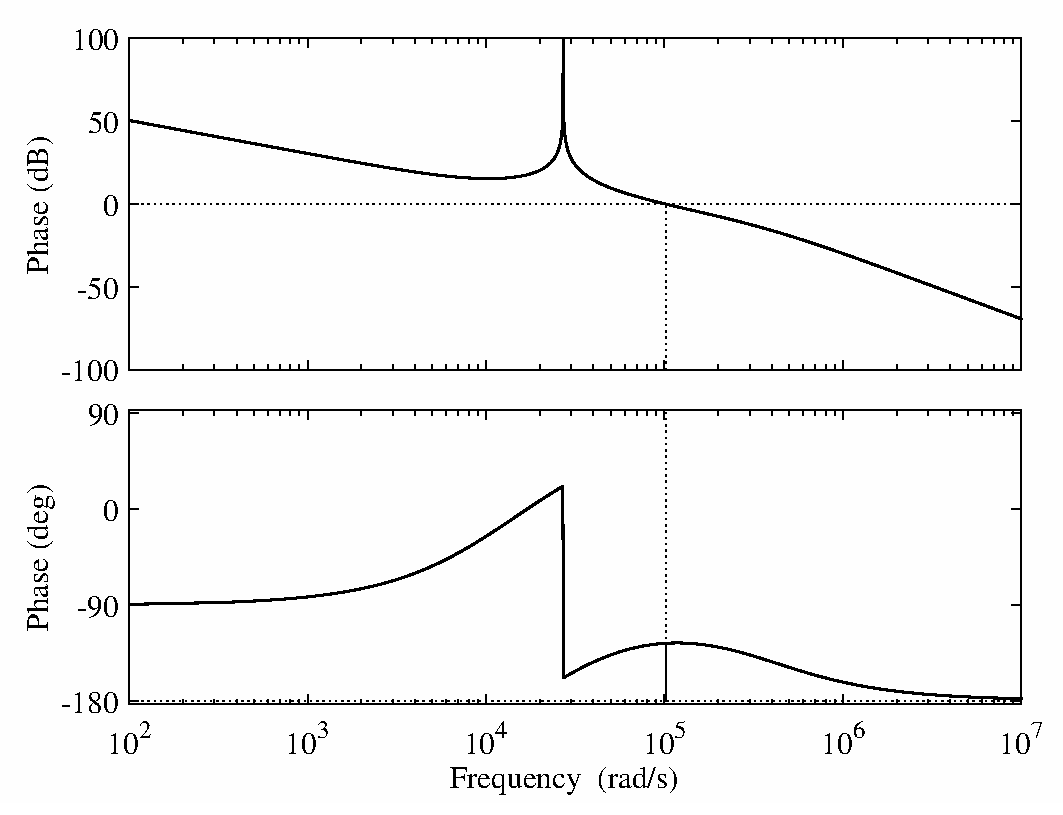
\includegraphics[width=0.45\textwidth]{compensated-vs}
		\caption{Bode plot of compensated transfer function of voltage source Gm = $\infty$,  Pm = 54.3$^\circ$ (at 1.02e+05 rad/s)}
		\label{fig:comp-vs}
	\end{figure}

	For the current source, phase margin is already sufficient, so closing the negative feedback loop with unity should be enough. This was verified in the simulation.

	\begin{comment}
	by designing a lead compensator such that the gain crossover frequency was increased as above. The bode plot for compensated open loop transfer function of the current source is shown in Fig. \ref{fig:comp-cs}. The slight increase in gain crossover frequency due to the compensator did not result in any significant change in the performance of the current source. Hence, the $Gc$ was kept as unity.

	\begin{figure}
		\centering
		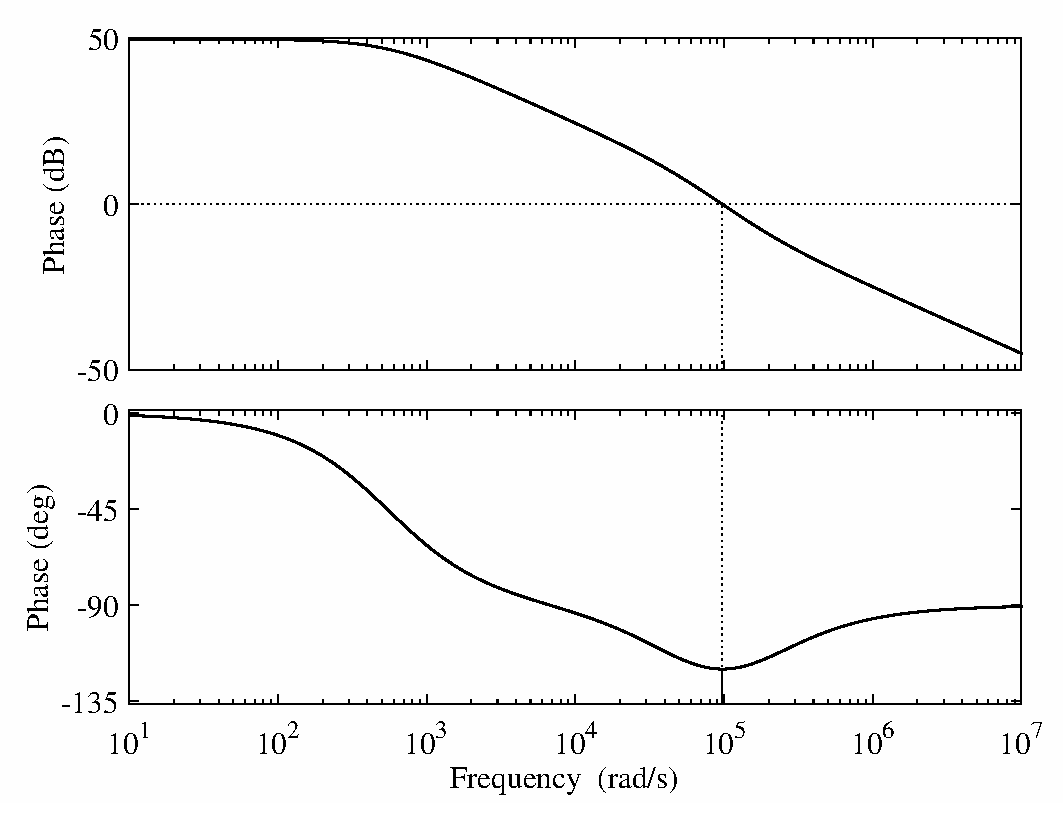
\includegraphics[width=0.45\textwidth]{compensated-cs}
		\caption{Bode plot of compensated transfer function of current source; Gm = $\infty$ ,  Pm = 60$^\circ$ (at 9.7e+04 rad/s)}
		\label{fig:comp-cs}
	\end{figure}
	\end{comment}

\subsection{Current Mode Control}
	Converters employing direct duty ratio control require a separate protection against over current for each switch. However, if the control method is based on the peak current through switch, then the requirement for such a protection effort is eliminated as the current is not allowed to rise above a particular threshold in each switching cycle. Also, the dynamics of such a controller are much simple than the direct duty ratio control. This section describes peak current mode control \cite{book:941109}, loosely referred to as current mode control, which employs this method to achieve the output current or voltage tracking objective.

	\begin{figure}
		\centering
		\includesvg[width=0.45\textwidth]{current-mode-minimal-master}
		\caption{Block diagram of current mode control of single quadrant converter}
		\label{fig:16}
	\end{figure}

	Fig. \ref{fig:16} represents the block diagram for current mode control of a single quadrant converter. At the start of each switching cycle of frequency $F_s$, $Q_1$ is switched on by a clock pulse which sets the latch in a high state. The switch remains in the on state until a reset pulse is applied to the latch. During on time, the current $i_s(t)$ through $Q_1$ rises with slope $m_1$ as shown in Fig. \ref{fig:17}. When $i_s(t)$ reaches the control current $i_c(t)$, the comparator, being non inverting in nature, generates a reset pulse for the latch which turns the switch off. For the remainder of the switching period, the current through switch is zero. If inductor $L$ is chosen such that the converter operates in continuous conduction mode around $i_c(t)$, then the current through the inductor decreases at a rate of $-m_2$ during the off time to a value of $i_L(T_S)$ at $T_s$ as shown in Fig. \ref{fig:18}.

	\begin{figure}
		\centering
		\includesvg[width=0.45\textwidth]{switch-current}
		\caption{Switch current in current mode control of single quadrant converter}
		\label{fig:17}
	\end{figure}

	\begin{figure}
		\centering
		\includesvg[width=0.45\textwidth]{inductor-current}
		\caption{Inductor current in current mode control of single quadrant converter}
		\label{fig:18}
	\end{figure}

	The slopes $m_1$ and $-m_2$ are given by

	\begin{align}
		m_1 = \dfrac{v_g-v}{L} \quad \text{and} \quad  -m_2=\dfrac{v}{L}
		\label{eq:1}
	\end{align}

	where $v_g$ is the dc link voltage, $v$ is the output voltage, and $L$ is the value of inductor of the buck converter.
	During on time, inductor current at $t=dT_s$, $\hat{i}_L(dT_s)$ in terms of slope $m_1$ is given by
	
	\begin{equation}
		i_L(dT_s) = i_c = i_L(0)+m_1dT_S
		\label{eq:2}
	\end{equation}

	During off time, inductor current at $t=T_s$ is 

	\begin{equation*}
		i_L(T_s) = i_L(dT_s) - m_2(1-d)T_S
	\end{equation*}

	Substituting $i_L(dT_s)$ from equation \eqref{eq:1} in this relation results in

	\begin{equation}
		i_L(T_s) = i_L(0)+m_1dT_S - m_2(1-d)T_S
		\label{eq:3}
	\end{equation}

	At steady state, $i_L(0) = i_L(T_s)$, $d=D$, $m_1=M_1$, and $m_2=M_2$. From equations \eqref{eq:2} and \eqref{eq:3}, at steady state

	\begin{equation*}
		0 = M_1DT_S - M_2(1-D)T_S
	\end{equation*}

	\begin{equation}
		\dfrac{M_2}{M_1} = \dfrac{D}{1-D}
		\label{eq:4}
	\end{equation}

	This method requires additional current sensing circuit as compared to duty ratio control methods, but in practice, duty ratio control methods also require current sensing circuit for protection against over currents. This method exploits the available current sensors which would otherwise be operating independently from the control scheme to achieve the control objective. Switch failures due to excessive currents are avoided by limiting the maximum value of control signal $i_c(t)$ thus ensuring that the switch will turn off when excessive current flows through it during each switching period.

	The only disadvantage of current mode control is its high susceptibility to noise. Perturbations in sensed switch current can cause premature turn off of the switch. Also, converter becomes unstable even for small perturbations in switch current when operating on duty cycles greater than 50\% as the perturbation increases in magnitude in each subsequent switching cycle. However, this can be remedied by adding an artificial ramp to the sensed switch current. The intuition behind this is explained in appendix \ref{app:instability-cmc}.

	\begin{figure}
		\centering
		\includesvg[width=0.45\textwidth]{current-mode-voltage-control}
		\caption{Controlled voltage source using current mode control}
		\label{fig:24}
	\end{figure}

	For the two quadrant converter, an outer voltage feedback loop is constructed on top the current mode controller as shown in Fig. \ref{fig:24}. A small signal model of the converter is derived under a justifiable assumption for this purpose. It is assumed that the current mode controller operates ideally, and hence causes the average inductor current ${i}_L$ to be identical to the control ${i}_c$.This approximation is justified whenever the inductor current ripple and artificial ramp have negligible magnitudes. The inductor current then is no longer an independent state of the system because $\dfrac{i_L}{i_c} \approx 1$. The current mode control part of this controller can be replaced by an ideal current source of magnitude $i_c(t)$ and an equivalent circuit can be constructed as shown in Fig. \ref{fig:25}

	\begin{figure}
		\centering
		\includesvg[width=0.4\textwidth]{modelling}
		\caption{Current mode control replaced as current source in buck converter}
		\label{fig:25}
	\end{figure}

	From Kirchhoff's Current Law, the output current of the current source is

	\begin{equation}
		i_c(t) = C\dfrac{dv(t)}{dt} + \dfrac{v(t)}{R}
		\label{eq:cmc-1}
	\end{equation}

	Let the steady state value of the output current and output voltage be $I_c$ and $V$ respectively. If a small perturbation of magnitude $\hat{i}_c(t)$ is introduced in the current $i_c(t)$, the output voltage $v(t)$ gets perturbed by a magnitude of, say, $\hat{v}(t)$, then

	\begin{align}
		i_c(t) &= I_c + \hat{i_c}(t)\\
		v(t) &= V + \hat{v}(t)
		\label{eq:cmc-2}
	\end{align}

	From \eqref{eq:cmc-1},

	\begin{equation}
		I_c + \hat{i_c}(t) = C\dfrac{d}{dt}(V + \hat{v}(t)) + \dfrac{V + \hat{v}(t)}{R}
		\label{eq:cmc-3}
	\end{equation}

	At the steady state, 

	\begin{equation}
		\dfrac{dV}{dt} = 0 \quad \text{and} \quad I_c = \dfrac{V}{R}
		\label{eq:cmc-4}
	\end{equation}

	Therefore,

	\begin{equation}
		\hat{i_c}(t) = C\dfrac{d\hat{v}(t)}{dt} + \dfrac{\hat{v}(t)}{R}
		\label{eq:cmc-5}
	\end{equation}

	Taking Laplace transform

	\begin{equation}
		\hat{i}_c(s) = sC\hat{v}(s) + \dfrac{\hat{v}(s)}{R}
	\end{equation}

	\begin{equation}
		\dfrac{\hat{v}(s)}{\hat{i}_c(s)} = \dfrac{R}{1+sRC}
	\end{equation}

	This transfer function represents first order dynamics. Thus, the simpler dynamics in comparison to models required for direct duty ratio control. A PI controller was used to complete the feedback loop to derive a controlled voltage source from a current mode controlled converter.

\section{Practical Considerations}
\label{sec:practical-considerations}
	This section deals with the methodology used to arrive at the capacitor and inductor sizes used for the simulation described in next section.

\subsection{Inductor Selection}
	The purpose of inductor in DC-DC switched power supplies is to maintain the current when the DC link switch is off i.e. to reduce the ripple in output voltage or current depending on the converter. With this criteria, the inductor value should be high, but when a large inductor is used, the rise time of converter is more as it takes more time for the current to rise. Hence, the selection of inductor is trade-off between the current ripple and transient response of the converter. 

	For the single quadrant converter which is used as current source, criteria for selection of inductor value is taken to be the the output current ripple of the converter. The relation between inductor value and the output current ripple \cite{book:768263} is 

	\begin{equation}
		\Delta I_L = \dfrac{V_{o1}}{L_1} (1-D) T_s
		\label{eq:ind-1}
	\end{equation}

	where $V_{o1} = I_{\text{ref}} R_L$ is the output voltage of the single quadrant converter, $L_1$ is the value of the inductor, $D$ is the steady state duty cycle of the converter, $\Delta I_L$ is the ripple in in inductor current and $T_s = \dfrac{1}{F_s}$ is the switching period.

	\begin{equation}
		L_1 \geq \dfrac{V_{o1}(V_d-V_{o1})}{\Delta I_L F_s V_d}
		\label{eq:ind-1a}
	\end{equation}

	Based on these calculations, inductor $L_1$ was chosen to be of 2 mH. 

	For the voltage source, the boundary condition for continuous conduction mode operation governs the choice of inductor. Because the output current need not be controlled here, the ripple criteria is relaxed in favour of inductor selection on the basis of continuous conduction mode operation. A buck converter operates in continuous conduction mode when the average inductor current satisfies \cite{book:768263}

	\begin{equation}
		I_{L_2} \geq \dfrac{DT_s}{2L_2}(V_d-V_{o2})
		\label{eq:ind-2}
	\end{equation}

	If the average inductor current $I_{L_{\text{avg}}}$ becomes less than this boundary value, the converter will operate in discontinuous mode. To extend the range of operation of the converter to lower average currents, the inductor is chosen such that continuous conduction mode is ensured at the lowest extreme of the intended range of operation. For satisfactory operation \cite{muhamad2005design} at $\dfrac{1}{5}I_{L_2}$, the condition in inequality \eqref{eq:ind-1} is

	\begin{equation}
		\dfrac{1}{5}I_{L_2} \geq \dfrac{DT_s}{2L_2}(V_d-V_{o2})
		\label{eq:ind-3}
	\end{equation}

	where $I_{L_2} = V_d / R_L$, $D$ is the steady state duty cycle, $T_s = 1 / F_s$ is the switching period, $L_2$ is the inductor value, and $V_d$ and $V_o = V_{\text{ref}}$ are the DC link and converter output voltages respectively. 
	Therefore,

	\begin{equation}
		L_2 \geq 2.5\dfrac{DT_s}{I_{L_2}}(V_d-V_{\text{ref}})
		\label{eq:ind-4}
	\end{equation}

	Based on this relation the inductor for voltage source was chosen to be 0.15 mH.

\subsection{Capacitor Selection}
	Capacitor is required in the output stage of two quadrant converter to filter out the output voltage ripple. For a ripple of $\Delta V_{o2}$, the value of capacitor required is given by\cite{book:768263}

	\begin{equation}
		C_2 \geq \dfrac{\Delta I_{L_2}T_s}{8\Delta V_{o2}}
		\label{eq:ind-4a}
	\end{equation}

	The current ripple is given by,

	\begin{equation}
		\Delta I_{L_2} \geq \dfrac{V_{o2}}{L_2}(1-D) T_s
		\label{eq:ind-4b}
	\end{equation}

	Here, $V_{o2} = V_{\text{ref}}$ and $T_s = 1 / F_s$,

	\begin{equation}
		C_2 \geq \dfrac{1 - D}{8 \dfrac{\Delta V_{o2}}{V_{\text{ref}}}L_2 F_s^2}
		\label{eq:ind-5}
	\end{equation}

	The capacitor was chosen to be of the value $10 \mu F$.

\subsection{Snubber Design}
	Snubber is required across the ignition switch $Q_d$ to limit the over-voltage arising due to opening of the switch. In highly inductive circuits, when switch is opened, the path for current flow is broken. Therefore, a high voltage spike appears on the switch terminals due to large magnitude of $L\dfrac{di}{dt}$. Energy absorbing circuit like the snubber circuit, reduces these spikes. This section explains the design procedure for a R-C snubber used in parallel with the ignition switch $Q_d$.

	The peak current through the snubber circuit is given by

	\begin{equation}
		I_p = \dfrac{V_{oc}}{R_s}
		\label{eq:snub-1}
	\end{equation}

	where $V_{OC}$ is the open circuit voltage across the switch, $R_s$ is the snubber resistance and $I_p$ is the peak current through the snubber.

	The current flowing through $Q_d$ before interruption is $I_{\text{ref}}$ and the maximum voltage across the terminals of $Q_d$ is $V_{\text{ref}}$. Hence, the snubber resistance $R_s$ should be minimum of

	\begin{equation}
		R_s \geq \dfrac{V_{\text{ref}}}{I_{\text{ref}}}
		\label{eq:snub-2}
	\end{equation}

	The snubber capacitance should be such that

	\begin{enumerate}
		\item Energy that is allowed to be stored in the capacitor should be greater than the energy stored in the inductor i.e.

			\begin{align}
				\dfrac{1}{2}C_sV_{oc}^2 &\geq \dfrac{1}{2}L_{eq}I_p^2\\
				\therefore C_s &\geq \dfrac{L_{eq}I_p^2}{V_{oc}^2}
				\label{eq:snub-3}
			\end{align}

		\item The time constant of the snubber circuit should be small as compared to the shortest on time of $Q_d$. So, for time constant of snubber circuit to be 10\% of the on time of $Q_d$

			\begin{align}
				R_sC_s &\leq \dfrac{T_{on}}{10}\\
				\therefore C_s &\leq \dfrac{T_{on}}{10R_s}
				\label{eq:snub-4}
			\end{align}
	\end{enumerate}

	From equations \eqref{eq:snub-2}, \eqref{eq:snub-3}, and \eqref{eq:snub-4}, $R_s$ was chosen $8 \Omega$ and $C_s$ was chosen as $2 \mu F$

\section{Results}
	The values of components derived in above section were used in a simulation of the converter with 50 kHz switching frequency and 5 kHz machining frequency. The voltage and current waveforms across the load when direct duty ratio control is used are shown in Fig. \ref{fig:1b}. 

	\begin{figure}
		\centering
		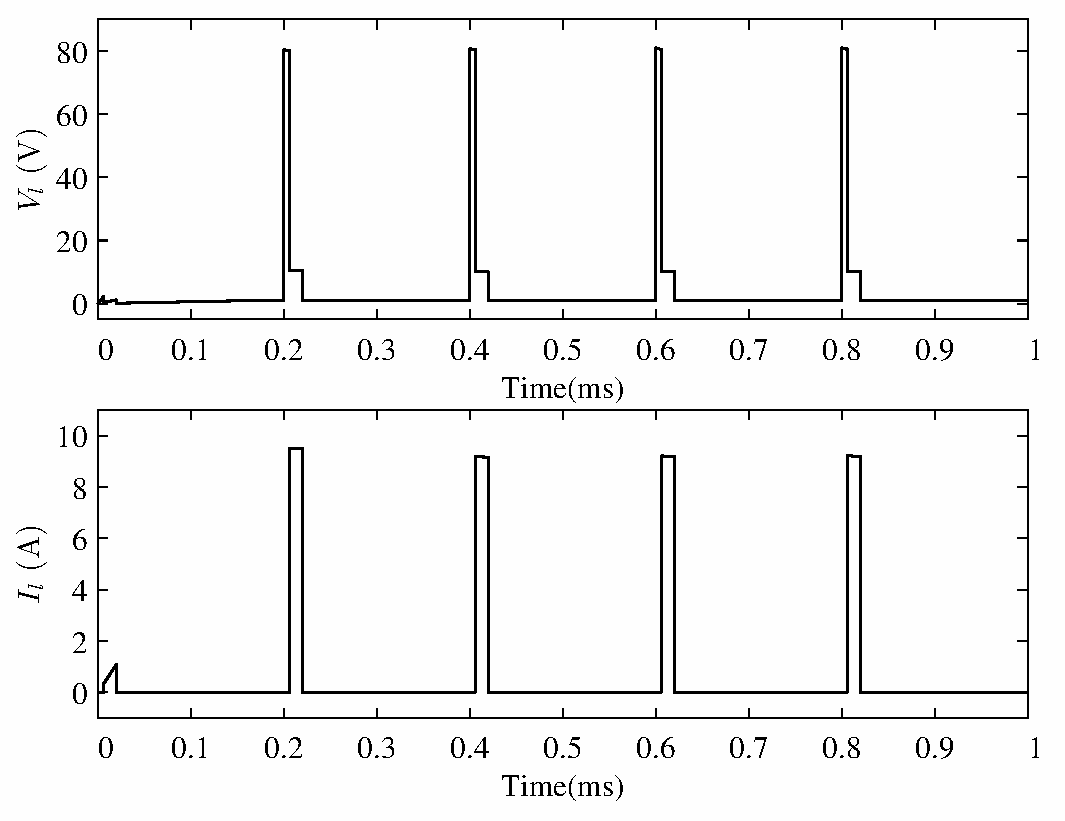
\includegraphics[width=0.45\textwidth]{load_comp}
		\caption{Load voltage and current - direct duty ratio control}
		\label{fig:1b}
	\end{figure}

	The output waveforms thus obtained are in well agreement with the results in \cite{tastekin2009novel}.

	Fig. \ref{fig:sim-qd} shows the voltage across $Q_d$ and current through $Q_d$ waveforms when direct duty ratio control is used. The maximum voltage across $Q_d$ is $V_{\text{ref}}$ i.e. 80 V and and the maximum current through $Q_d$ is 11 A during the rise time.

	\begin{figure}
		\centering
		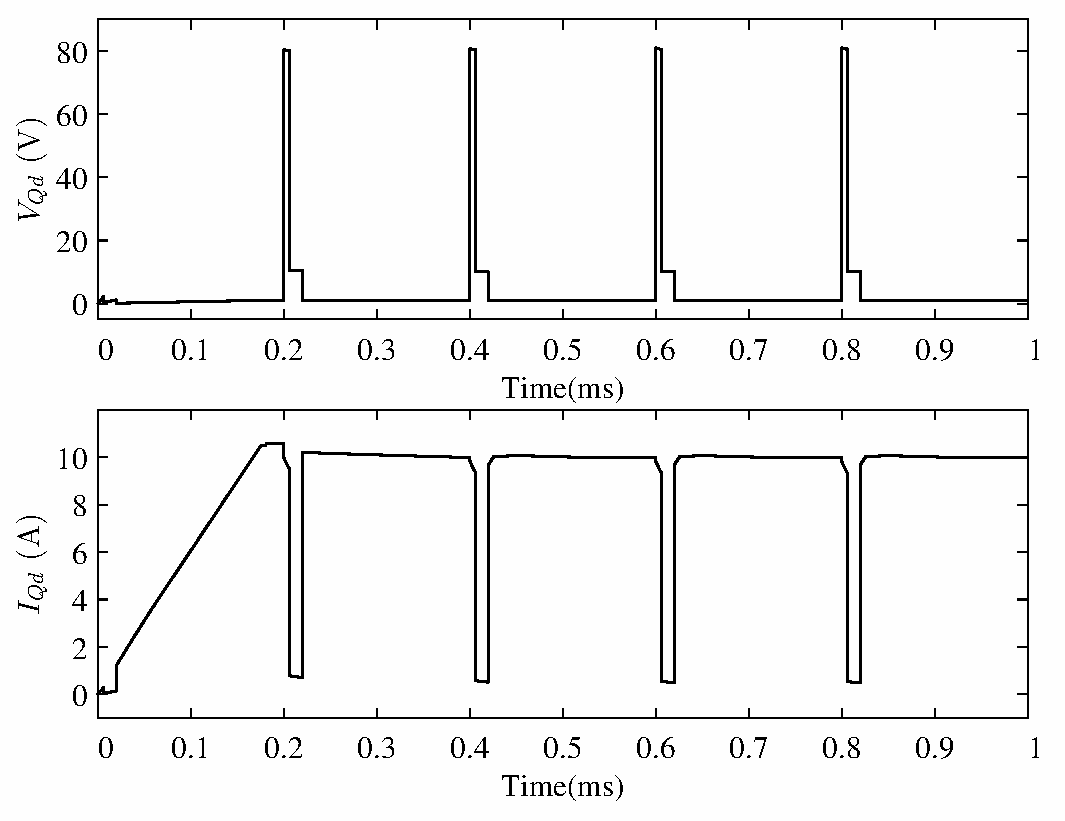
\includegraphics[width=0.45\textwidth]{Qd}
		\caption{Voltage and current of Qd - direct duty ratio control}
		\label{fig:sim-qd}
	\end{figure}

	Fig. \ref{fig:sim-d} shows the voltage across $D$ and current through $D$ waveforms when direct duty ratio control is used. The maximum reverse voltage across $D$ is 83 V and the maximum forward current through it is 0.8 A.

	\begin{figure}
		\centering
		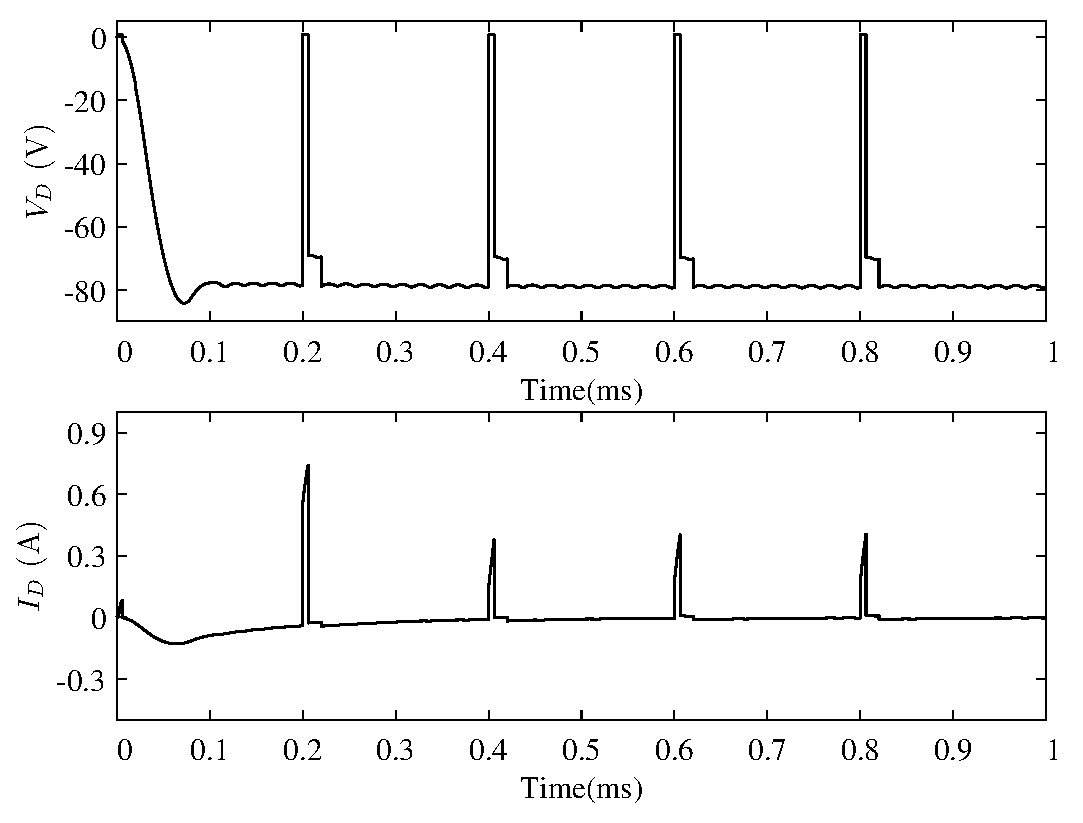
\includegraphics[width=0.45\textwidth]{D}
		\caption{Voltage and current of D - direct duty ratio control}
		\label{fig:sim-d}
	\end{figure}

	Fig. \ref{fig:sim-q1} shows the voltage across $Q_1$ and current through $Q_1$ waveforms when direct duty ratio control is used. The maximum voltage across $Q_1$ is $V_d$ i.e 110 V and the maximum current through it is 11 A.

	\begin{figure}
		\centering
		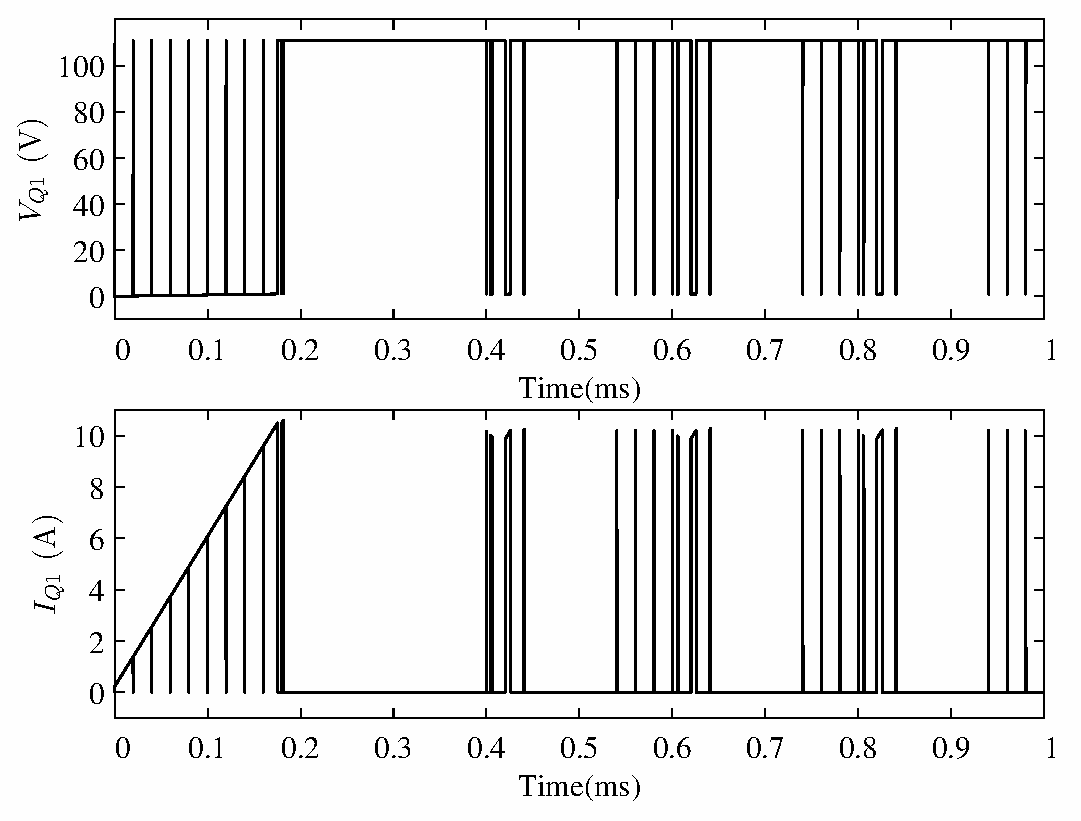
\includegraphics[width=0.45\textwidth]{Q1}
		\caption{Voltage and current of Q1 - direct duty ratio control}
		\label{fig:sim-q1}
	\end{figure}

	Fig. \ref{fig:sim-d1} shows the voltage across $D_1$ and current through $D_1$ waveforms when direct duty ratio control is used. The maximum reverse voltage across diode $D_1$ is $V_d$ i.e. 110 V and the maximum forward current through it is 11 A.

	\begin{figure}
		\centering
		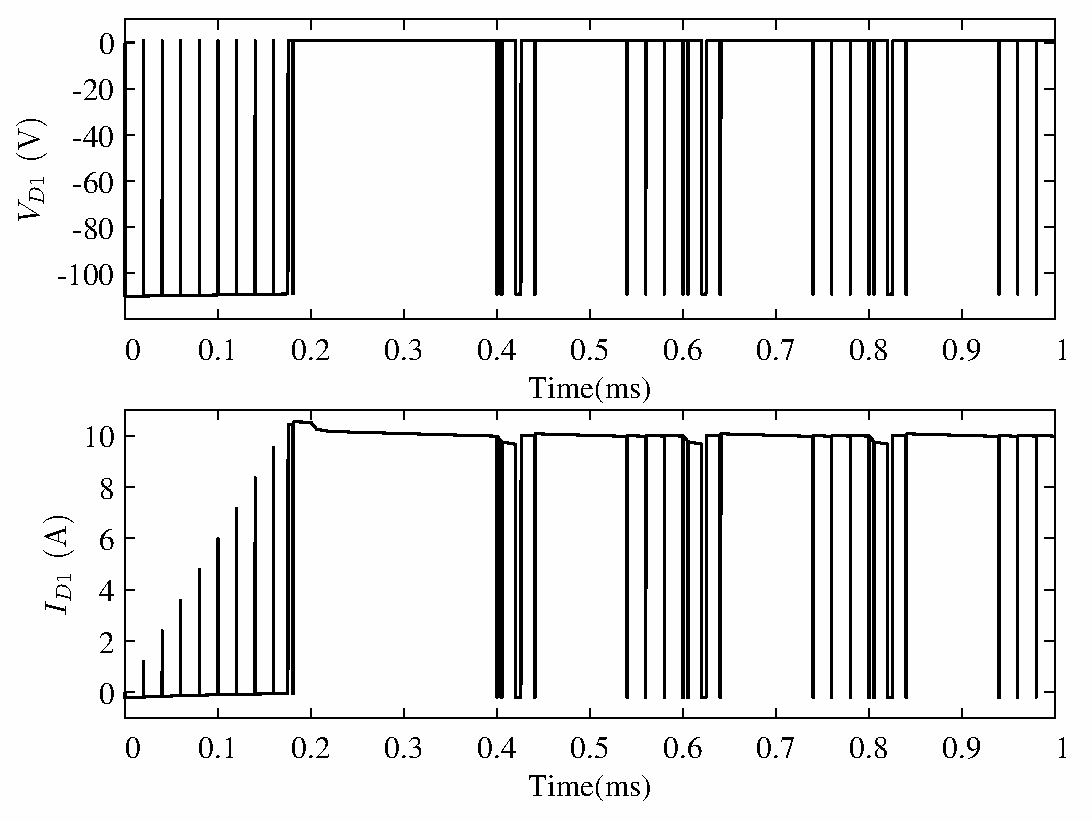
\includegraphics[width=0.45\textwidth]{D1}
		\caption{Voltage and current of D1 - direct duty ratio control}
		\label{fig:sim-d1}
	\end{figure}

	Fig. \ref{fig:sim-q2} shows the voltage across $Q_2$ and current through $Q_2$ waveforms when direct duty ratio control is used. The maximum voltage across $Q_2$ is $V_d$ i.e 110 V and the maximum current through it is 21 A. This maximum occurs during the rise time of the voltage source.

	\begin{figure}
		\centering
		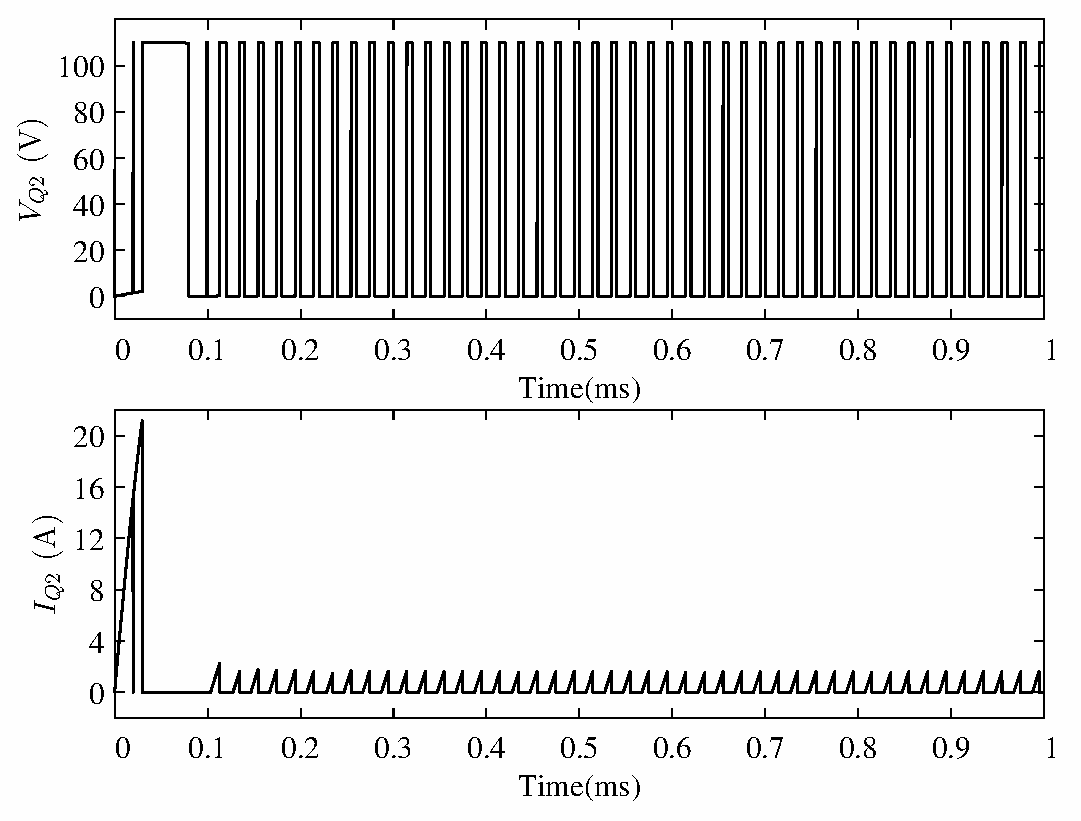
\includegraphics[width=0.45\textwidth]{Q2}
		\caption{Voltage and current of Q2 - direct duty ratio control}
		\label{fig:sim-q2}
	\end{figure}

	Fig. \ref{fig:sim-d2} shows the voltage across $D_2$ and current through $D_2$ waveforms when direct duty ratio control is used. The maximum reverse voltage across $D_2$ is $V_d$ i.e. 110 V and the maximum current through it is 4.5 A.

	\begin{figure}
		\centering
		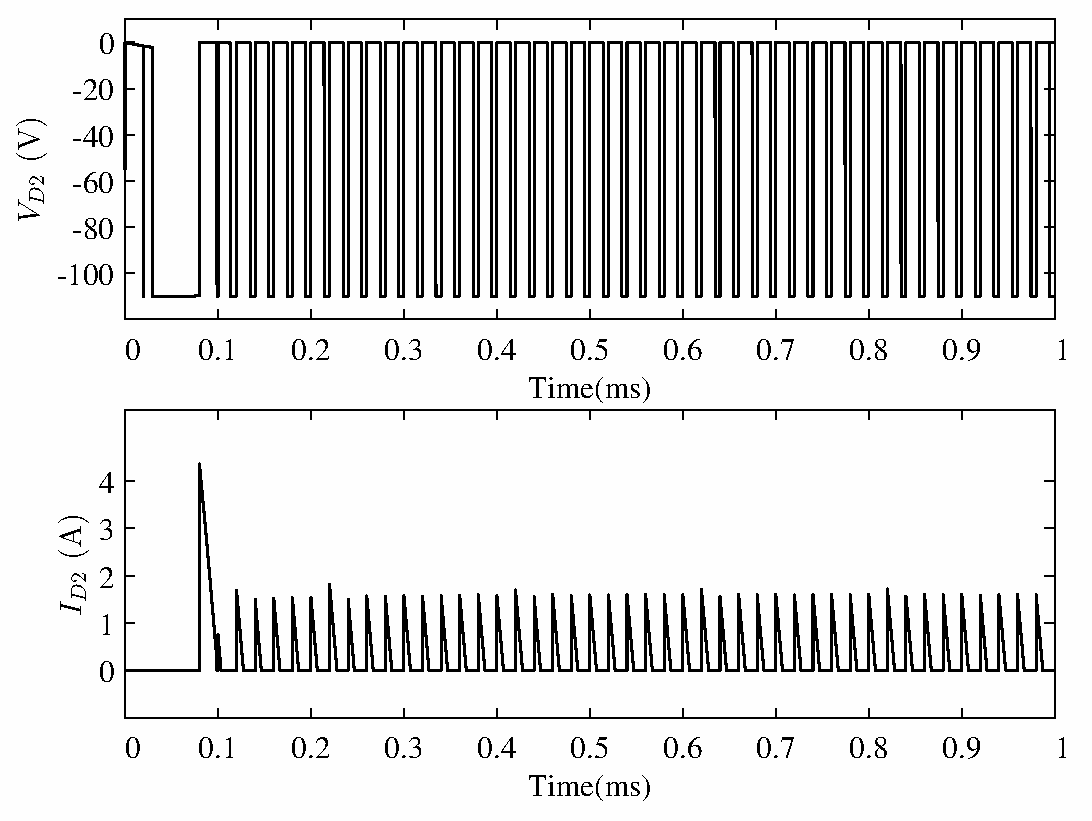
\includegraphics[width=0.45\textwidth]{D2}
		\caption{Voltage and current of D2 - direct duty ratio control}
		\label{fig:sim-d2}
	\end{figure}

	Fig. \ref{fig:sim-q3} shows the voltage across $Q_3$ and current through $Q_3$ waveforms when direct duty ratio control is used. The maximum voltage across $Q_3$ is 110 V and the maximum current through it is 4.5 A. 

	\begin{figure}
		\centering
		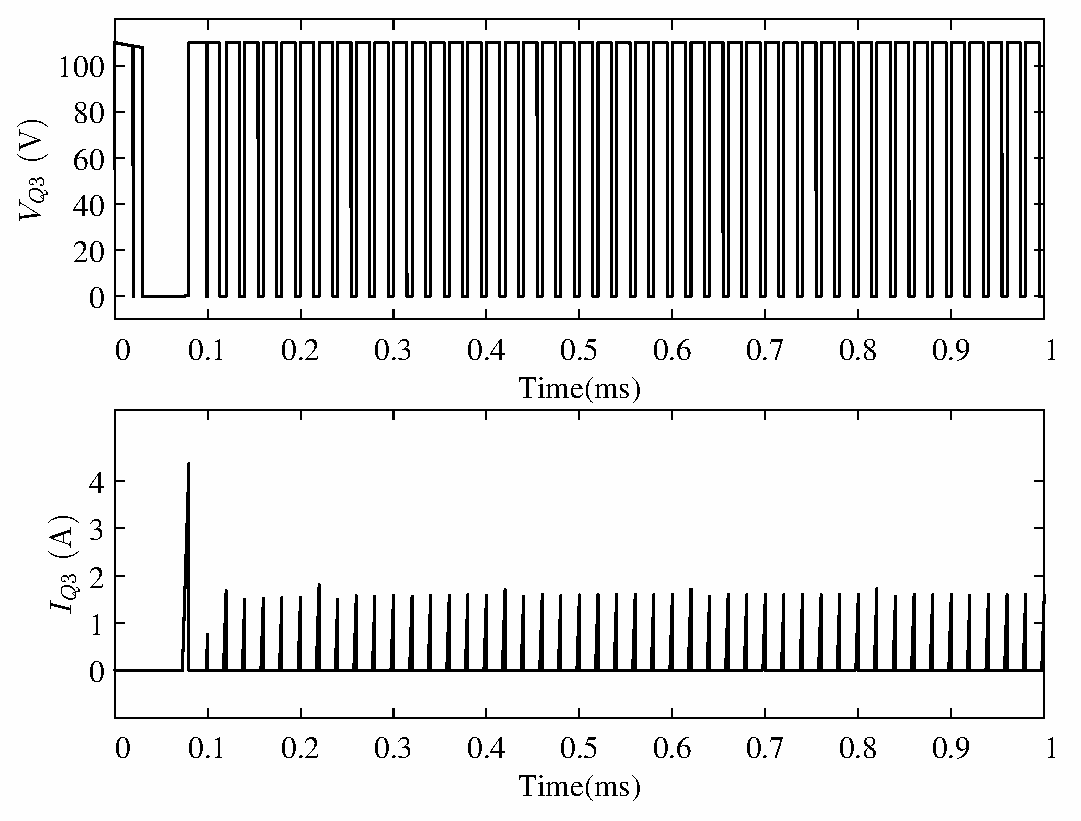
\includegraphics[width=0.45\textwidth]{Q3}
		\caption{Voltage and current of Q3 - direct duty ratio control}
		\label{fig:sim-q3}
	\end{figure}

	Fig. \ref{fig:sim-d3} shows the voltage across $D_3$ and current through $D_3$ waveforms when direct duty ratio control is used. The maximum reverse voltage across $D_3$ is 110 V and the maximum current through it is 21 A.

	\begin{figure}
		\centering
		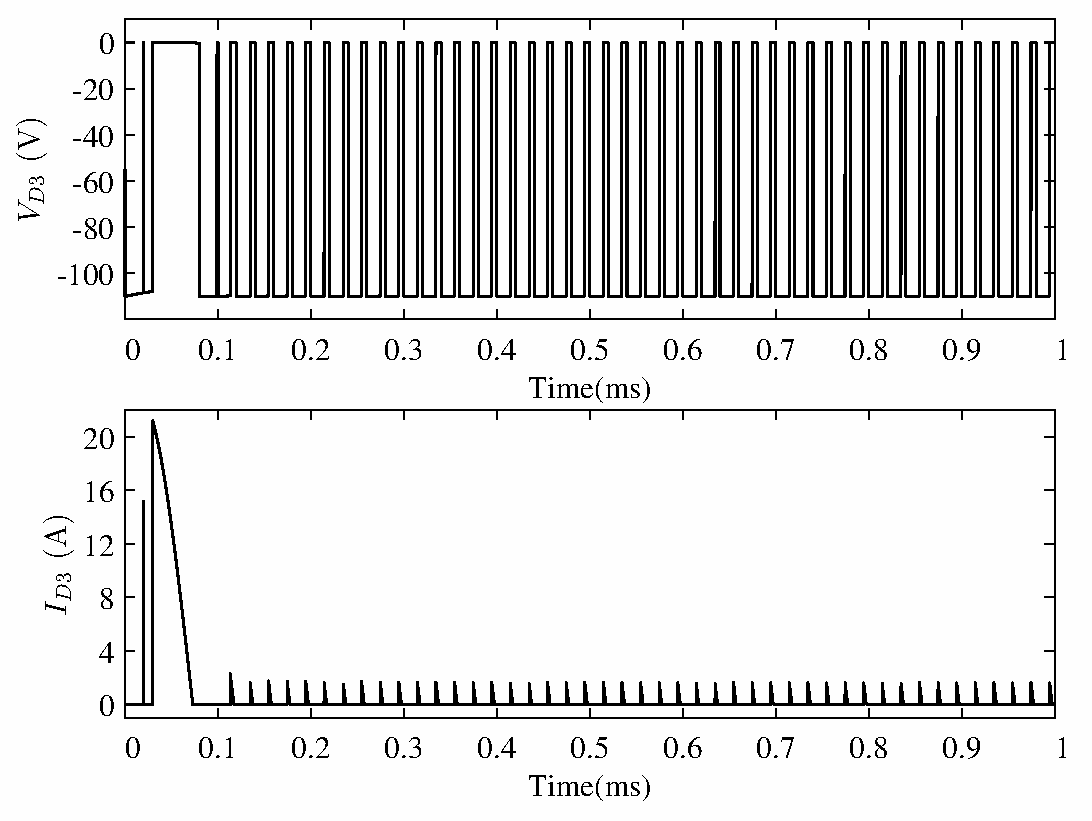
\includegraphics[width=0.45\textwidth]{D3}
		\caption{Voltage and current of D3 - direct duty ratio control}
		\label{fig:sim-d3}
	\end{figure}

	Fig. \ref{fig:sim-cmc} shows the load voltage and current waveforms when current mode control is used.

	\begin{figure}
		\centering
		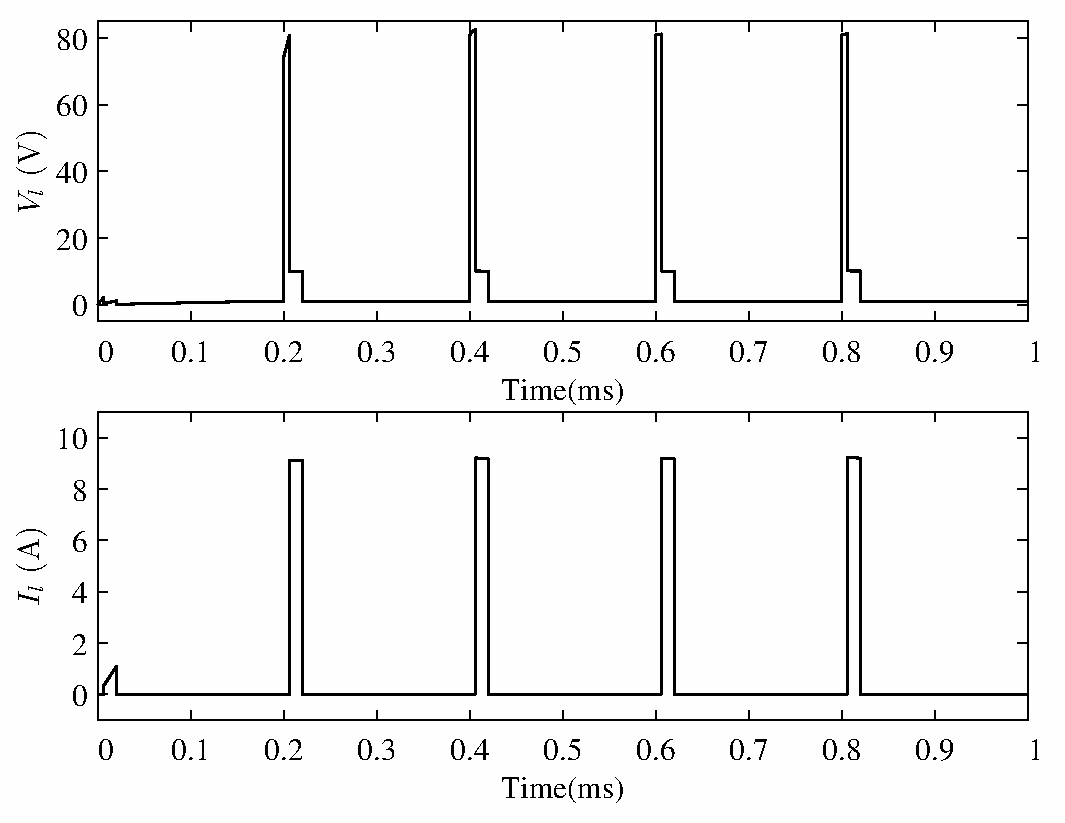
\includegraphics[width=0.45\textwidth]{load_cmc}
		\caption{Load voltage and current - current mode control}
		\label{fig:sim-cmc}
	\end{figure}

\section{Future Plan}
\subsection{Fabrication of Power Supply}
	The power supply design has been completed and the next step would be designing the PCBs and Gate drivers. Once these are done, the power supply could be assembled. The testing of power supply is to be done with the spark gap jar available in the Insulation Diagnostics lab. The X-Y slides were ordered previous to match the specifications required for further experimentation. These have now arrived and and can be used to make a desktop EDM setup for further experimentation.

\subsection{Load Modelling}
	The electrical characterisation of the spark gap load is to be done. Previous research has established that spark gaps can be represented as parallel combination of R, L and C elements. The further experimentation would be directed towards fitting a model or approximating these values directly to obtain a load model. This will help in better understanding and also to highlight any scope for improvement in the power supply.

\bibliography{../references/references}
\bibliographystyle{IEEEtran}


\appendices

\section{Time Averaging Modelling Technique}
\label{app:modelling}
	The large signal representation of voltage source in Fig. \ref{fig:working-4} as derived in equation \eqref{eq:mod14}

	\begin{equation*}
		\begin{split}
			\dot{x} &= [dA_1+(1-d)A_2]x + [dB_1 + (1-d)B_2]V_d\\
			V_o &= [dC_1+(1-d)C_2]x
		\end{split}
	\end{equation*}	

	Introducing small perturbations in $x$, $V_o$ and $d$ as

	\begin{equation}
		\begin{split}
			x &= X + \hat{x}\\
			v_o &= V_o + \hat{v_o}\\
			d &= D + \hat{d}
		\end{split}
		\label{eq:mod15}
	\end{equation} 
	
	Since the transfer function is to be determined between $\hat{v_o}$ and $\hat{d}$, perturbations in $v_d$ are assumed to be zero for simplicity, therefore
	
	\begin{equation}
		v_d = V_d
		\label{eq:mod16}
	\end{equation}
	
	Using the fact that at steady state $\dot{X} = 0$ and the equations \eqref{eq:mod15} in equation \eqref{eq:mod14}
	
	\begin{multline}
		\dot{\hat{x}} = AX + BV_d + A\hat{x} + [(A_1-A_2)X+(B_1-B_2)V_d]\hat{d} \\+ \text{terms with products of $\hat{x}$ and $\hat{d}$ (neglected)} 
		\label{eq:mod17}
	\end{multline}
	
	where
	
	\begin{align}
		A &= A_1D+A_2(1-D)\\
		B &= B_1D+B_2(1-D)
		\label{eq:mod18}
	\end{align}
	
	At steady state, the perturbations in equation \eqref{eq:mod17} are zero, therefore
	
	\begin{equation}
		AX+BV_d=0
		\label{eq:mod19}
	\end{equation}
	
	Hence, when perturbations are introduced in a converter operating under steady state
	
	\begin{equation}
		\dot{\hat{x}} = A\hat{x} + [(A_1-A_2)X+(B_1-B_2)V_d]\hat{d}
		\label{eq:mod20}
	\end{equation}

	Similarly, for output voltage, using equations \eqref{eq:mod15} in equation \eqref{eq:mod14}
	
	\begin{equation}
		V_o + \hat{v}_o = CX + C\hat{x} + [(C_1-C_2)X]\hat{d}
		\label{eq:mod21}
	\end{equation}
	
	where
	
	\begin{equation}
		C = C_1D+C_2(1-D)
		\label{eq:mod22}
	\end{equation}
	
	At steady state

	\begin{equation}
		V_o = CX
		\label{eq:mod23}
	\end{equation}
	
	Hence, when perturbations are introduced in a converter operating under steady state
		\begin{equation}
		\hat{v}_o = C\hat{x}+[(C_1-C_2)X]\hat{d}
		\label{eq:mod24}
	\end{equation}
	
	Taking Laplace transform of equation \eqref{eq:mod20}
	
	\begin{align}
		s\hat{x}(s) &= Ax(s)+[(A_1-A_2)X+(B_1-B_2)V_d]\hat{d}(s)\\
		\therefore \hat{x}(s) &= [sI-A]^{-1}[(A_1-A_2)X+(B_1-B_2)V_d]\hat{d}(s)
		\label{eq:mod25}
	\end{align}
	
	where $I$ is a unity matrix
	Taking Laplace transform of equation \eqref{eq:mod24}
	
	\begin{equation}
		\hat{v}_o(s) = C\hat{x}(s)+[(C_1-C_2)X]\hat{d}(s)
		\label{eq:mod26}
	\end{equation}
	
	Substituting in $\hat{x}(s)$ from equation \eqref{eq:mod25}
	
	\begin{multline}
		\hat{v}_o(s) = \{C[sI-A]^{-1}[(A_1-A_2)X+(B_1-B_2)V_d]\\+(C_1-C_2)X\}\hat{d}(s)
		\label{eq:mod27b}
	\end{multline}

	\begin{multline}
		\therefore \dfrac{\hat{v}_o(s)}{\hat{d}(s)} = C[sI-A]^{-1}[(A_1-A_2)X+(B_1-B_2)V_d]\\+(C_1-C_2)X
		\label{eq:mod27}
	\end{multline}

	This is the small signal transfer function of the output voltage of two quadrant converter with respect to the duty ratio of the switch $Q_2$

\section{Instability in Current Mode Control}
\label{app:instability-cmc}
	Consider the waveform of steady state switch current as shown in Fig. \ref{fig:19} for a buck converter operating at duty cycle $D>0.5$. A small perturbation $\hat{i}_L(0)$ such that $|\hat{i}_L(0)| << |i_L(0)|$ is introduced in inductor current $i_L(t)$ which same as the switch current $i_s(t)$ at time $t=0$. During on time, the perturbed inductor current rises with slope of $m_1$ till time $(D+\hat{d})T_s$. At this instant, perturbed $i_L(t)=i_c(t)$ and the switch turns off. For the remainder of switching signal, $i_L(t)$ decreases with slope $-m_2$, and at $t=T_s$ the perturbation in inductor current is $\hat{i}_L(T_s)$. 

	\begin{figure}
		\centering
		\includesvg[width=0.45\textwidth]{wf-no-ramp}
		\caption{Inductor current in presence of disturbance}
		\label{fig:19}
	\end{figure}

	Fig. \ref{fig:20} is the expanded view of perturbed and steady state inductor current between times $(D+\hat{d})T_s$ and $T_s$. Inductor current at time $t=0$ is given by

	\begin{equation*}
		i_L(0) = i_{L0} + \hat{i}_L(0)
	\end{equation*}

	The perturbation in inductor current at $t=0$ and $t=T_s$ are given by

	\begin{align}
		\hat{i}_L(0) &= -m_1\hat{d}T_s\\
		\hat{i}_L(T_s) &= m_2\hat{d}T_s\\
		\hat{i}_L(T_s) &= \hat{i}_L(0) \left( -\dfrac{m_2}{m_1} \right)
		\label{eq:5}
	\end{align}

	From relation governing slopes $m_1$ and $m_2$ in equation \eqref{eq:4},

	\begin{align}
		\hat{i}_L(T_s) &= \hat{i}_L(0) \left( -\dfrac{D}{1-D} \right)
		\label{eq:6}
	\end{align}

	At each cycle the perturbation will magnify by a factor of $\dfrac{D}{1-D}$, therefore, after $n$ such switching cycles, the perturbation in inductor current is

	\begin{equation}
		i_L(nT_s) = i_L(0)\left( -\dfrac{D}{1-D} \right)^n
		\label{eq:7}
	\end{equation}

	Thus, the magnification of initial perturbation depends on the duty ratio of the switch operation. If $D<0.5$, then the magnification factor $|\dfrac{D}{1-D}| < 1$, and any initial perturbations in the inductor or switch current will eventually die down. But, if $D>0.5$, then $|\dfrac{D}{1-D}| > 1$, the perturbations will only increase in magnitude with time, irrespective of the initial magnitude of the perturbation. Thus,

	\begin{align}
		|\hat{i}_L(nT_s)| \longrightarrow \left\{ 
		\parbox[]{2in}
		{$0 \quad \text{when} \quad \left|-\dfrac{D}{1-D}\right| < 1 $\\
		$\infty \quad \text{when} \quad \left|-\dfrac{D}{1-D}\right| > 1$}
		\right.
		\label{eq:8}
	\end{align}

	\begin{figure}
		\centering
		\includesvg[width=0.45\textwidth]{expanded-no-ramp}
		\caption{Expanded view of perturbed inductor current}
		\label{fig:20}
	\end{figure}

	In this form, the satisfactory operation of converter is limited to a range $0 \leq D \leq 0.5$. To overcome this limitation, an artificial ramp $i_a(t)$ with slope $m_a$ and frequency equal to the switching frequency $F_s$ is added with the switch current as shown in Fig. \ref{fig:21}. Due to the addition of this ramp, the controller causes the switch to turn off when

	\begin{equation*}
		i_a(t) + i_L(t) = i_c
	\end{equation*}

	i.e.

	\begin{equation}
		i_L(t) = i_c - i_a(t)
		\label{eq:9}
	\end{equation}

	\begin{figure}
		\centering
		\includesvg[width=0.45\textwidth]{current-mode-ramp}
		\caption{Block diagram of current mode control with artificial ramp compensation}
		\label{fig:21}
	\end{figure}

	\begin{figure}
		\centering
		\includesvg[width=0.45\textwidth]{wf-ramp}
		\caption{Inductor current with artificial ramp in presence of disturbance}
		\label{fig:22}
	\end{figure}

	Fig. \ref{fig:22} shows the steady state and perturbed current waveforms for buck converter operating at duty $D>0.5$ in presence of initial perturbation $\hat{i}_L(0)$. From Fig. \ref{fig:23}, the initial disturbance in terms of slopes $m_1$ and $m_a$ is

	\begin{equation}
		\hat{i}_L(0) = -\hat{d}T_s(m_1+m_a)
		\label{eq:10}
	\end{equation}

	\begin{equation}
		\hat{i}_L(T_s) = -\hat{d}T_s(m_a-m_2)
		\label{eq:11}
	\end{equation}

	Therefore,

	\begin{equation}
		\hat{i}_L(T_s) = \hat{i}_L(0)\left(-\dfrac{m_2-m_a}{m_1+m_a} \right)
		\label{eq:12}
	\end{equation}

	The magnification in perturbation after $n$ switching cycles is
	Therefore,

	\begin{equation}
		\hat{i}_L(nT_s) = \hat{i}_L(0)\left(-\dfrac{m_2-m_a}{m_1+m_a} \right)^n
		\label{eq:13}
	\end{equation}

	When $n\longrightarrow \infty$,

	\begin{align}
		|\hat{i}_L(nT_s)| \longrightarrow \left\{ 
		\parbox[]{2in}
		{$0 \quad \text{when} \quad |\alpha| < 1 $\\
		$\infty \quad \text{when} \quad |\alpha| > 1$}
		\right.
		\label{eq:14}
	\end{align}

	where $$ \alpha = -\dfrac{m_2-m_a}{m_1+m_a} $$

	\begin{figure}
		\centering
		\includesvg[width=0.45\textwidth]{expanded-ramp}
		\caption{Expanded view of inductor current with artificial ramp in presence of disturbance}
		\label{fig:23}
	\end{figure}

	For stable operation of converter, the slope of the artificial ramp $m_a$ such that the magnification factor $|\alpha| < 1$. $\alpha$ from can be rearranged as

	\begin{equation}
		\alpha = -\dfrac{1-\dfrac{m_a}{m_2}}{\dfrac{1-D}{D}+\dfrac{m_a}{m_2}}
		\label{eq:15}
	\end{equation}

	If $m_a$ is chosen such that $m_a = \dfrac{1}{2}m_2$, then from equation \eqref{eq:15} $\alpha = -1$ at $D = 1$ and $|\alpha|<1$ for $0 \leq D < 1$. This is the minimum slope required for artificial ramp to stabilise the operation of converter over all operating duties. If $m_a$ is chosen such that $m_a = m_2$, then $\alpha$ is zero for all $D$. Therefore, $\hat{i}_L(T_s)$ is $0$ for any $\hat{i}_L(0)$. Thus, the system has finite settling time and removes any perturbation after one switching period $T_s$.

\end{document}

% Debug info
% ==========
% Inkscape Test:
% runsystem("C:/Program Files/Inkscape/inkscape.com" -z -D  --file="../working/RepresenatativeDiagram1.svg" --export-pdf="RepresenatativeDiagram1_svg-raw.pdf" )
% texify test
% texify -b -p --engine=pdftex --tex-option="--synctex=1" --tex-option="--shell-escape" report.tex
